\documentclass[conference]{IEEEtran}
\IEEEoverridecommandlockouts
% The preceding line is only needed to identify funding in the first footnote. If that is unneeded, please comment it out.
\usepackage{cite}
\usepackage{amsmath,amssymb,amsfonts}
\usepackage{algorithmic}
\usepackage{graphicx}
\usepackage{textcomp}
\usepackage{xcolor}
\usepackage[font=small,justification=centering]{caption}
\usepackage{subcaption}
%\usepackage{appendix}
\def\BibTeX{{\rm B\kern-.05em{\sc i\kern-.025em b}\kern-.08em
    T\kern-.1667em\lower.7ex\hbox{E}\kern-.125emX}}
\begin{document}

\title{Human Mask Generation in Images\\
\thanks{Identify applicable funding agency here. If none, delete this.}
}

\author{\IEEEauthorblockN{Gursimar Singh}
\IEEEauthorblockA{\textit{B.Tech (Final Year), Department of Electronics and Communication Engineering} \\
\textit{PDPM Indian Institute of Information Technology, Design and Manufacturing, Jabalpur}\\
gursimarsingh@iiitdmj.ac.in}
}

\maketitle

\begin{abstract}
Pixel-wise segmentation of objects in natural environments is one of the most discussed problems of modern times in computer vision. Many object detectors gained both popularity and accuracy after state-of-the-art object localization deep learning algorithms were introduced. But a bounding box is not enough for many applications and thus pixel-wise segmentation is required. My work was focused on pixel-wise accurate mask generation of humans in images. I explored and experimented various conventional image processing and modern deep learning models for this task. Human mask generation can be eased if we have information about the pose of the human to be segmented. This not only helps in providing a prior/seed for segmentation but also helps to identify the person in focus in an image. This report summarizes the pros and cons of various approaches. Analysis of each approach has also been done on fixed person dataset from MS-COCO 2017 and PASCAL VOC 2012.\\ 
\end{abstract}
\begin{IEEEkeywords}
Segmentation, Human Pose, Convolution Neural Networks, Conditional Random Fields
\end{IEEEkeywords}

\section{INTRODUCTION}
This document is a model and instructions for \LaTeX.
Please observe the conference page limits. 

\section{LITERATURE REVIEW}

Human mask generation can be modelled as a different problem than that of generic object segmentation. Here, we can take advantage of the essential keypoints of the human body thatrepresent the pose of human body. This pose information tells us about the structure of the human body and thus facilitate segmentation. Previous works where pose information is used for human parsing include the Joint Body-Parsing and Keypoint Estimation Network \cite{jppNet}. This novel joint human parsing and pose estimation network incorporates the multiscale feature connections and iterative location refinement in an end-to-end framework. It detects keypoints as well as generate mask and it has been used as a one of the evaluation baselines in this report. 
 
\subsection{Deep Matching and Deep Flow} \label{DM}

Deep Match is a 6-layer convolution-based algorithm which finds dense correspondences between two images. It was introduced in \cite{deepmatch}. Deep Matching relies on a deep, multi-layer, convolutional architecture designed for matching images. It can handle non-rigid deformations and repetitive textures, can therefore efficiently determine dense correspondences in the presence of significant changes between images. It convolves the inpur frames in 4x4 patches at multiple levels and thus forming a multiscale pyramid of the actiavtion maps. ``Fig. \ref{fig:dm_net}'' illustrates the process flow of the algorithm.

Deep Flow is an optical flow algorithm based on Deep Match. It computes the flow vectors of each pixel of the query image with respect to the reference image. For the subsequent frames of a video sequences there were about 95\% correspondences detected for each pair.
\begin{figure}[htbp]
\centerline{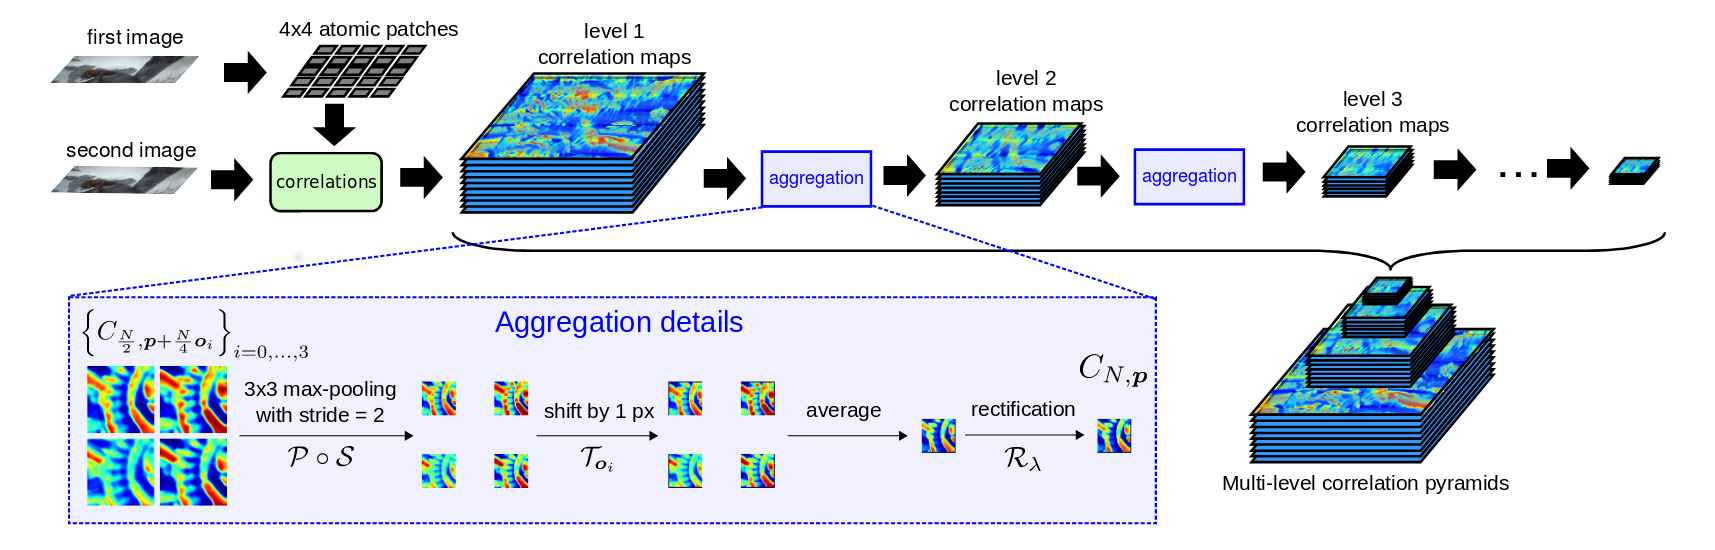
\includegraphics[width=\linewidth]{dm_net}}
\caption{Computing the Multi-level correlation pyramid}
\label{fig:dm_net}
\end{figure}

\subsection{Joint Body Parsing and Keypoint Estimation Network} \label{jpp}
It is a deep convolution neural network which estimates keypoints as well as generate mask for the human body. The mask generated are pixel-wise accurate. The output mask is divided into 20 semantic categories including background. The 19 foreground categories include 6 body parts and 13 clothing categories. From literature study and analysis of the existing approaches the author of JPP Net came up with two conclusions:
\begin{enumerate}
  \item The existing human does not consider human body configuration, meanwhile the information produced by the parsing network can also guide the locations joints
   \item A coarse-to-fine technique used in both parsing and pose networks. In case of parsing networks, it implies using multi-scale features for more precise pixel wise classification.
\end{enumerate} 

The architecture of the network is shown in ``Fig. \ref{fig:JPP_arch}''. The network uses Res-4 and Res-5 from ResNet-101 initially to extract feature maps from input image which are fed to the joint module and parsing module. The results generated are separate and can be obtained individually during inference.
\begin{figure}[htbp]
\centerline{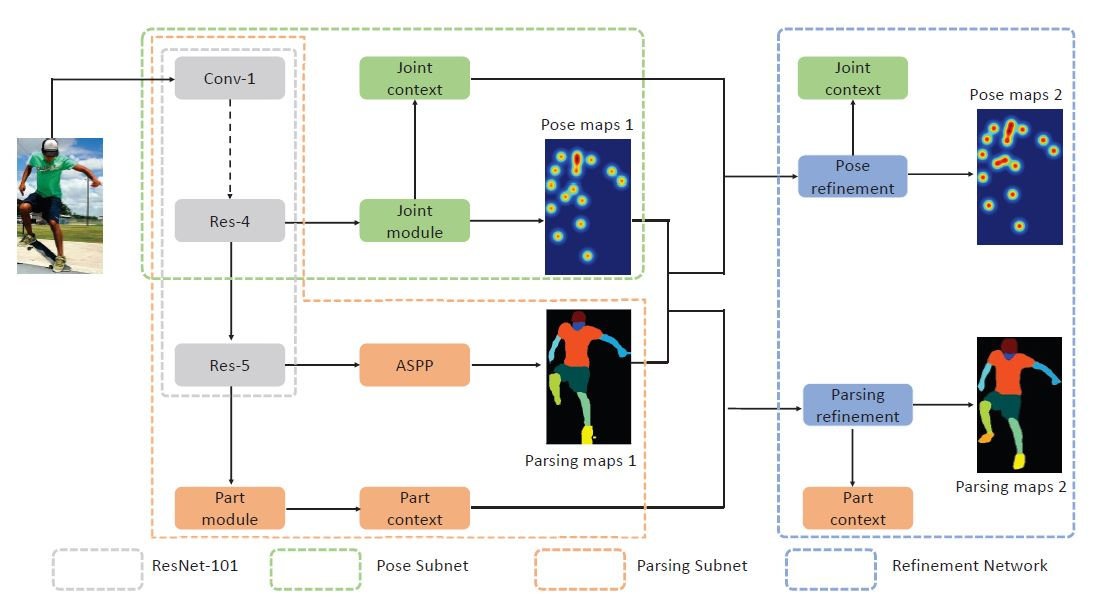
\includegraphics[width=\linewidth]{jpp_net}}
\caption{JPP-Net Architecture}
\label{fig:JPP_arch}
\end{figure} 
\subsection{Simple Linear Iterative Clustering}
Simple Linear Iterative Clustering \cite{slic} is an algorithm for dividing a image into segments/clusters known as superpixels. A superpixel is a group of pixels having similar characteristics. It is generally color based segmentation. It is based on a spatial localized version of k-means clustering. Each pixel is associated with a 5D feature vector as Eq. \ref{eq:1}\begin{align}\label{eq:1} \Psi  & = \begin{bmatrix} \lambda x\\ \lambda y\\ L(x,y) \\ a(x,y)\\b(x,y)\end{bmatrix} \end{align}
Here, x,y are the spatial coordinates of the pixels, $L(x,y), a(x,y), b(x,y)$ are the coressponding CIELAB color values and $\lambda$ is the regularizing parameter.  SLIC has two input parameters: Size of the regions $(S)$ and strength of spatial regularization $(m)$. The image is divided into grids and grid centers are used to initialize K-Means algorithm. During K-Means it aslo assumed that pixels associated with a cluster lie within $2S\times 2S$ area around the superpixel center in the xy plane, where $S$ is the size of the grid. The parameter regularizer sets the trade-off between clustering appearance and spatial regularization. This is obtained by setting 
\begin{equation} \lambda = m/S 
\end{equation} in the definition of the feature $\Psi(x,y)$. Therefore, the distance metric used while clustering is \begin{equation} D_{s} = d_{lab} + \lambda \times d_{xy}\end{equation} instead the euclidean distance over the 5D vector. An example of clustering is shown in ``Fig. \ref{fig:slic}''. 

\subsection{Gaussian Mixture Models and Expectation Maxmization}
Gaussian Mixture model is a very popular method for color based image segmentations. In this we model the color distribution of the image into a set of gaussians with different means and variances. Therefore, we obtain a model that fits the color distribution of the image. An example of the model fit is shown in ``Fig. \ref{fig:gmm}''.  

\begin{figure}[htbp]
\centering{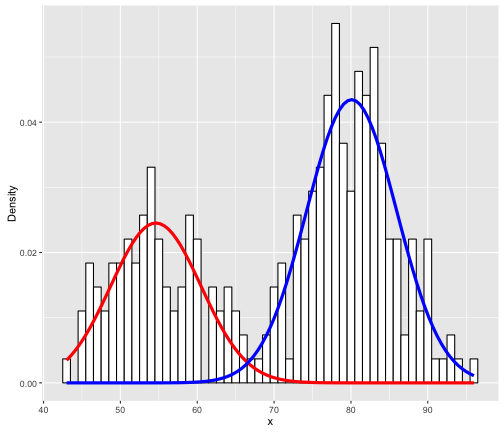
\includegraphics[width=0.9\linewidth]{gmm}}
\caption{Two Gaussians fitting the data in 1-Dimension}
\label{fig:gmm}
\end{figure}


\subsection{Graph Cut and Cooperative Cut} \label{gc}
Graph cut model the image segmentation problem as an energy minimization problem. There is a sink node and a source node to which all the pixels are connected. The edges are weighted with the probability for each node to belong to the sink/source node. Probabilities are found using the Gaussian foreground and background model which act as edge weights. After this a min cut/max flow algorithm cuts the graph into two parts namely background foreground. A representation of the algorithm is shown in ``Fig. \ref{fig:graph_cut}''.


Cooperative cut \cite{CoopCut} is an inference method for Markov Random Field (MRF) problem similar to Graph Cut. It introduces a penalizing parameter α for the edges. For image segmentation, this means cooperative cut encourages coherent boundaries, therefore preserving them.
\begin{figure}[htbp]
\centering{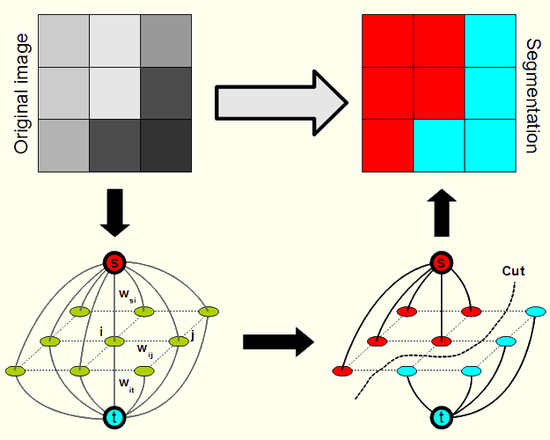
\includegraphics[width=0.9\linewidth]{graph_cut}}
\caption{Graph Cut Segmentation}
\label{fig:graph_cut}
\end{figure}


\subsection{U-Net architecture for image segmentation } \label{un}
U-Net was originally used in \cite{unet} .For biomedical image segmentation. It is an encoder-decoder network with symmetric skip connections. The features from the input image are first extracted using a fully convolutional encoder. The scaled down features are then deconvolved and concatenated in the decoder. After regular interval concatenation of the extracted features and reconstructed features is done using the skip connections. The network arhcitecture is shown in ``Fig. \ref{fig:unet}.'' \\

\begin{figure}[htbp]
\centering{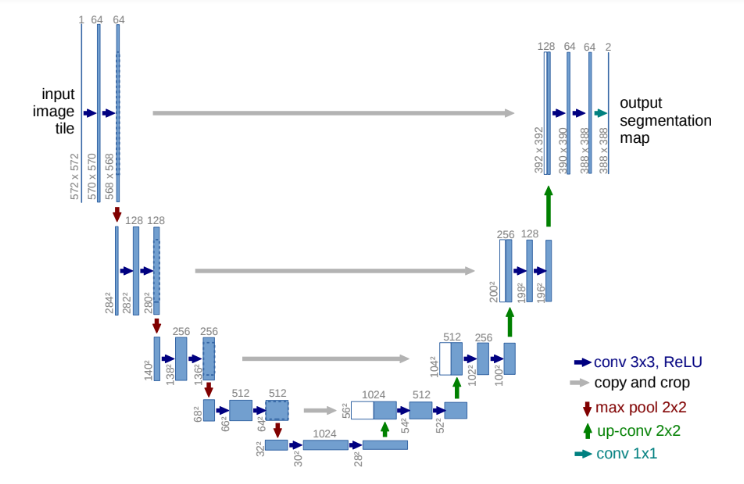
\includegraphics[width=\linewidth]{U-net}}
\caption{U-Net architecture}
\label{fig:unet}
\end{figure}

\section{METHODS}
In order to solve the task of mask generation various methods including conventional algorithms and deep learning approaches were explored. A summary of some of them are mentioned in the following sections. 

\subsection{Keypoint Tracking}
The task of mask generation also involved keypoint tracking in sequence of images for reducing annotation effort in correcting generated keypoints from keypoint detectors like \cite{poseAE}.

The basic approach to track keypoints used was matching features around those keypoints in subsequent frames. Various algorithms like SIFT \cite{sift}, ORB \cite{orb} are available for extracting relevant keypoints and compute their descriptors. But in order to compute descriptors for some specific keypoints open-source implementations of these algorithms cannot be used. Therefore, ORB being open-source algorithm was used by manually providing the keypoints to track and then computing its descriptors. However, this approach did not give good results especially when one or two frames were missing from the sequence. 

Therefore, Deep Match (see section \ref{DM}) was used to find matches between two subsequent frames. As the correspondences found were very dense, the chance that the human keypoints in one frame have corresspondences in other frame was very high. Even if a match for the particluar keypoint was not found, mean of the location of the points lying in its small radius was selected. Kalman Filter was then applied to these predictions in order to facilitate tracking. Sample results are demonstrated in ``Fig. \ref{fig:dm}''.

\begin{figure}[htbp]
\centering{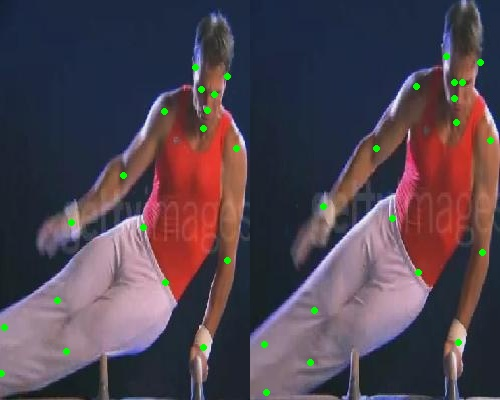
\includegraphics[width=0.9\linewidth]{dm1}}
\caption{ Keypoint Tracking in subsequent frames. \\ \textit{Left:} Reference frame, \textit{Right:} Query Frame.}
\label{fig:dm}
\end{figure}

\subsection{Graph Cut and Cooperative Cut}\label{gcm}

``Graph Cut and Cooperative Cut'' (see section \ref{gc}) are unsupervised techniques in which seeds are provided for the foreground and background region. The algorithm then model the RGB/LAB values of these seeds into foreground and backgorund Gaussian Mixture Models(GMM). The probabilities obtained for every pixel in the image from the GMM model act as unaries for the graph cut/cooperative cut algorithm algorithm. In our case seed for the foreground and background was obtained from the keypoint infoemation. A skeleton mask made by joining the keypoints in fixed order acted as foreground and the same skeleton mask with very bigger radius acted as background seed. For robust segementation an ensemble of ``SLIC'' (see section \ref{slic}) and Graph Cut is used. The intersection of the skeleton mask and the slic clusters make up the foreground seed. 

\begin{figure}[htbp]{}
\centering
\begin{subfigure}[t]{2cm}
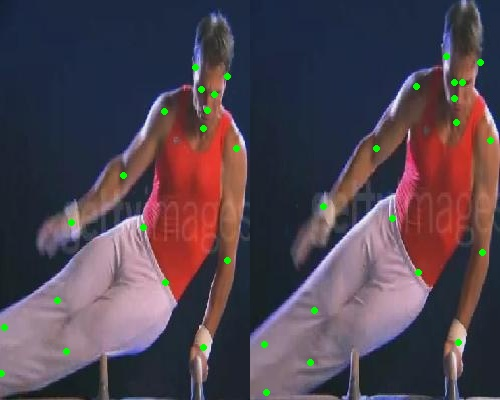
\includegraphics[width=\linewidth, height=1.2\linewidth]{dm1} 
\caption{Input peppers image}
\label{cari1}
\end{subfigure}
\hfill % some horizontal space
\begin{subfigure}[t]{2cm}
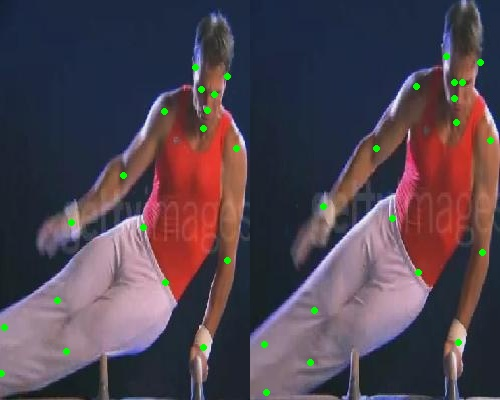
\includegraphics[width=\linewidth, height=1.2\linewidth]{dm1}
\caption{Reconstructed Peppers Image, M=20, PSNR = 30.9370 dB} 
\label{caro1}
\end{subfigure}
\hfill % some horizontal space
\begin{subfigure}[t]{2cm}
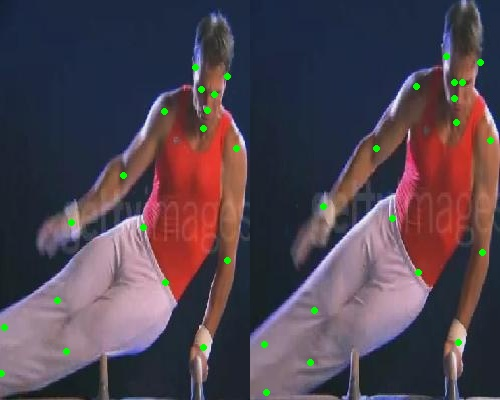
\includegraphics[width=\linewidth, height=1.2\linewidth]{dm1}
\caption{Reconstructed Peppers Image, M=20, PSNR = 30.9370 dB} 
\label{caro2}
\end{subfigure}
\hfill % some horizontal space
\begin{subfigure}[t]{2cm}
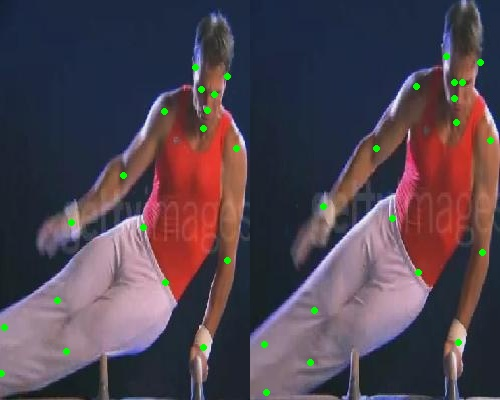
\includegraphics[width=\linewidth, height=1.2\linewidth]{dm1}
\caption{Reconstructed Peppers Image, M=20, PSNR = 30.9370 dB} 
\label{caro3}
\end{subfigure}
\caption{Reconstructed images and video frames using NITRA with 
number of measurements and their corresponding PSNR in dB}
\label{NITRAres1} 
\end{figure}

\subsection{Human Mask Generation Network}
It is an encoder-decoder network with skip connections inspired from the ``U-Net'' (see section \ref{un}) architecture. This network was a part of the segmentation module of ``posewarp'' (see section \ref{posew}). ``Posewarp'' is a modular generative adversial network that synthesizes unseen poses using training pairs of images and poses taken from human action videos. The network separates a scene into different body part and background layers, moves body parts to new locations and refines their appearances, and composites the new foreground with a hole-filled background. Our model is inspired from the ``Module-A'' that is image source segmentation module of this network.
\subsubsection{Pose Representation}
In the past works on pose representation \cite{poseAE}, human pose is represented by a set of joints. There are many different set of datasets available having different set of points. MS-COCO dataset \cite{coco} has 17 keypoints and LSP dataset \cite{lsp} has 14 keypoints. They majorily differ in the number of facial keypoints. In our model we use 14 joints namely head, neck, shoulders, elbows, wrists,hips,knees and ankles. $p_{s}$ is represented as 2D volume in $\mathbb{R}^{H\times W\times 1}$ where $H$ and $W$ are the height and width of the source image. Each keypoint is a Gaussian ``bump'' centered at the $(x, y)$ location of the keypoint. This representation allows the network to quickly leverage the spatial nature of the pose input in contrast to a flattened, dense representation. The spatial Gaussians also act as a regularization on the pose estimates which can be useful when joint locations
are noisy.

\subsubsection{Head Keypoint estimation}
Associative embedding \cite{poseAE} generates 17 keypoints. Also MS-COCO dataset has 17 keypoints (refer \ref{coco_l} for labels) that does not include the head. Therefore, head point is estimated from the locations of other facial points like eyes, ears, nose and neck. Estimation is done using a set of if-else conditions based on the availability of the keypoints. Three fundamental things that define a point; direction , a reference point and distance from the refrence point needs to be determined. Some of the examples are illustrated in ``Fig. \ref{head}''.
\begin{figure}[htbp]{}
\centering
\begin{subfigure}[t]{1.6cm}
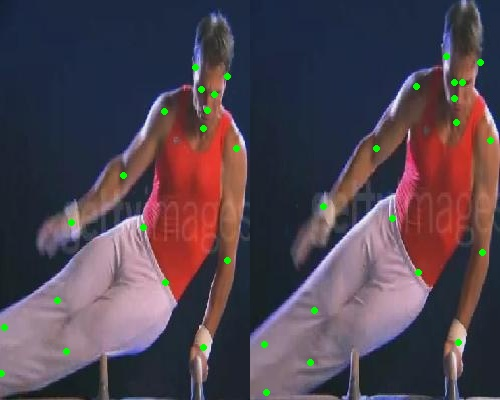
\includegraphics[width=\linewidth, height=\linewidth]{dm1} 
\caption{Input peppers image}
\label{cari1}
\end{subfigure}
%\hfill % some horizontal space
\begin{subfigure}[t]{1.6cm}
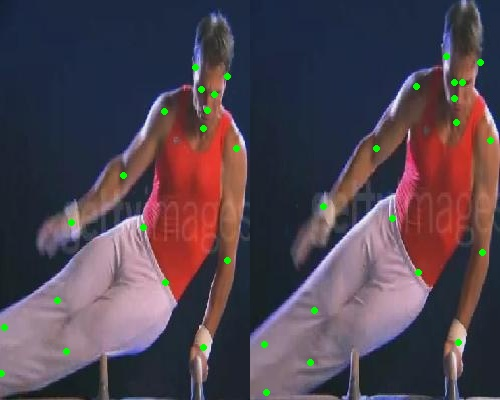
\includegraphics[width=\linewidth, height=\linewidth]{dm1}
\caption{Reconstructed Peppers Image, M=20, PSNR = 30.9370 dB} 
\label{caro1}
\end{subfigure}
%\hfill % some horizontal space
\begin{subfigure}[t]{1.6cm}
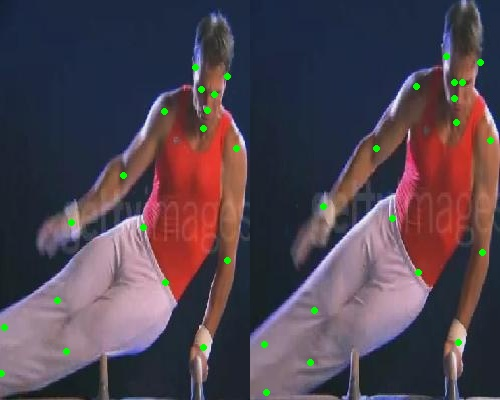
\includegraphics[width=\linewidth, height=\linewidth]{dm1}
\caption{Reconstructed Peppers Image, M=20, PSNR = 30.9370 dB} 
\label{caro2}
\end{subfigure}
%\hfill % some horizontal space
\begin{subfigure}[t]{1.6cm}
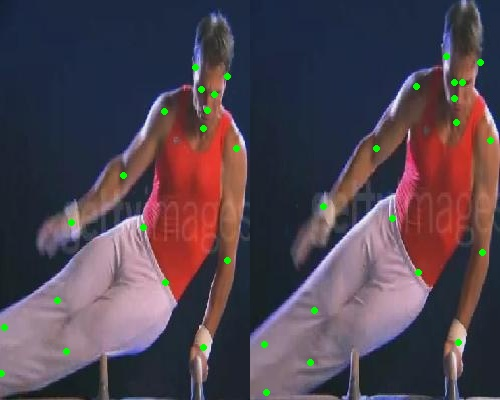
\includegraphics[width=\linewidth, height=\linewidth]{dm1}
\caption{Reconstructed Peppers Image, M=20, PSNR = 30.9370 dB} 
\label{caro3}
\end{subfigure}
\begin{subfigure}[t]{1.6cm}
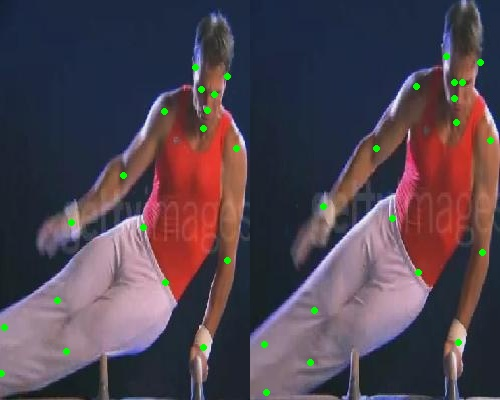
\includegraphics[width=\linewidth, height=\linewidth]{dm1}
\caption{Reconstructed Peppers Image, M=20, PSNR = 30.9370 dB} 
\label{caro3}
\end{subfigure}
\caption{Head point estimation}
\label{NITRAres1} 
\end{figure}

\subsubsection{The Model}
\begin{figure*}[htbp]
\centering{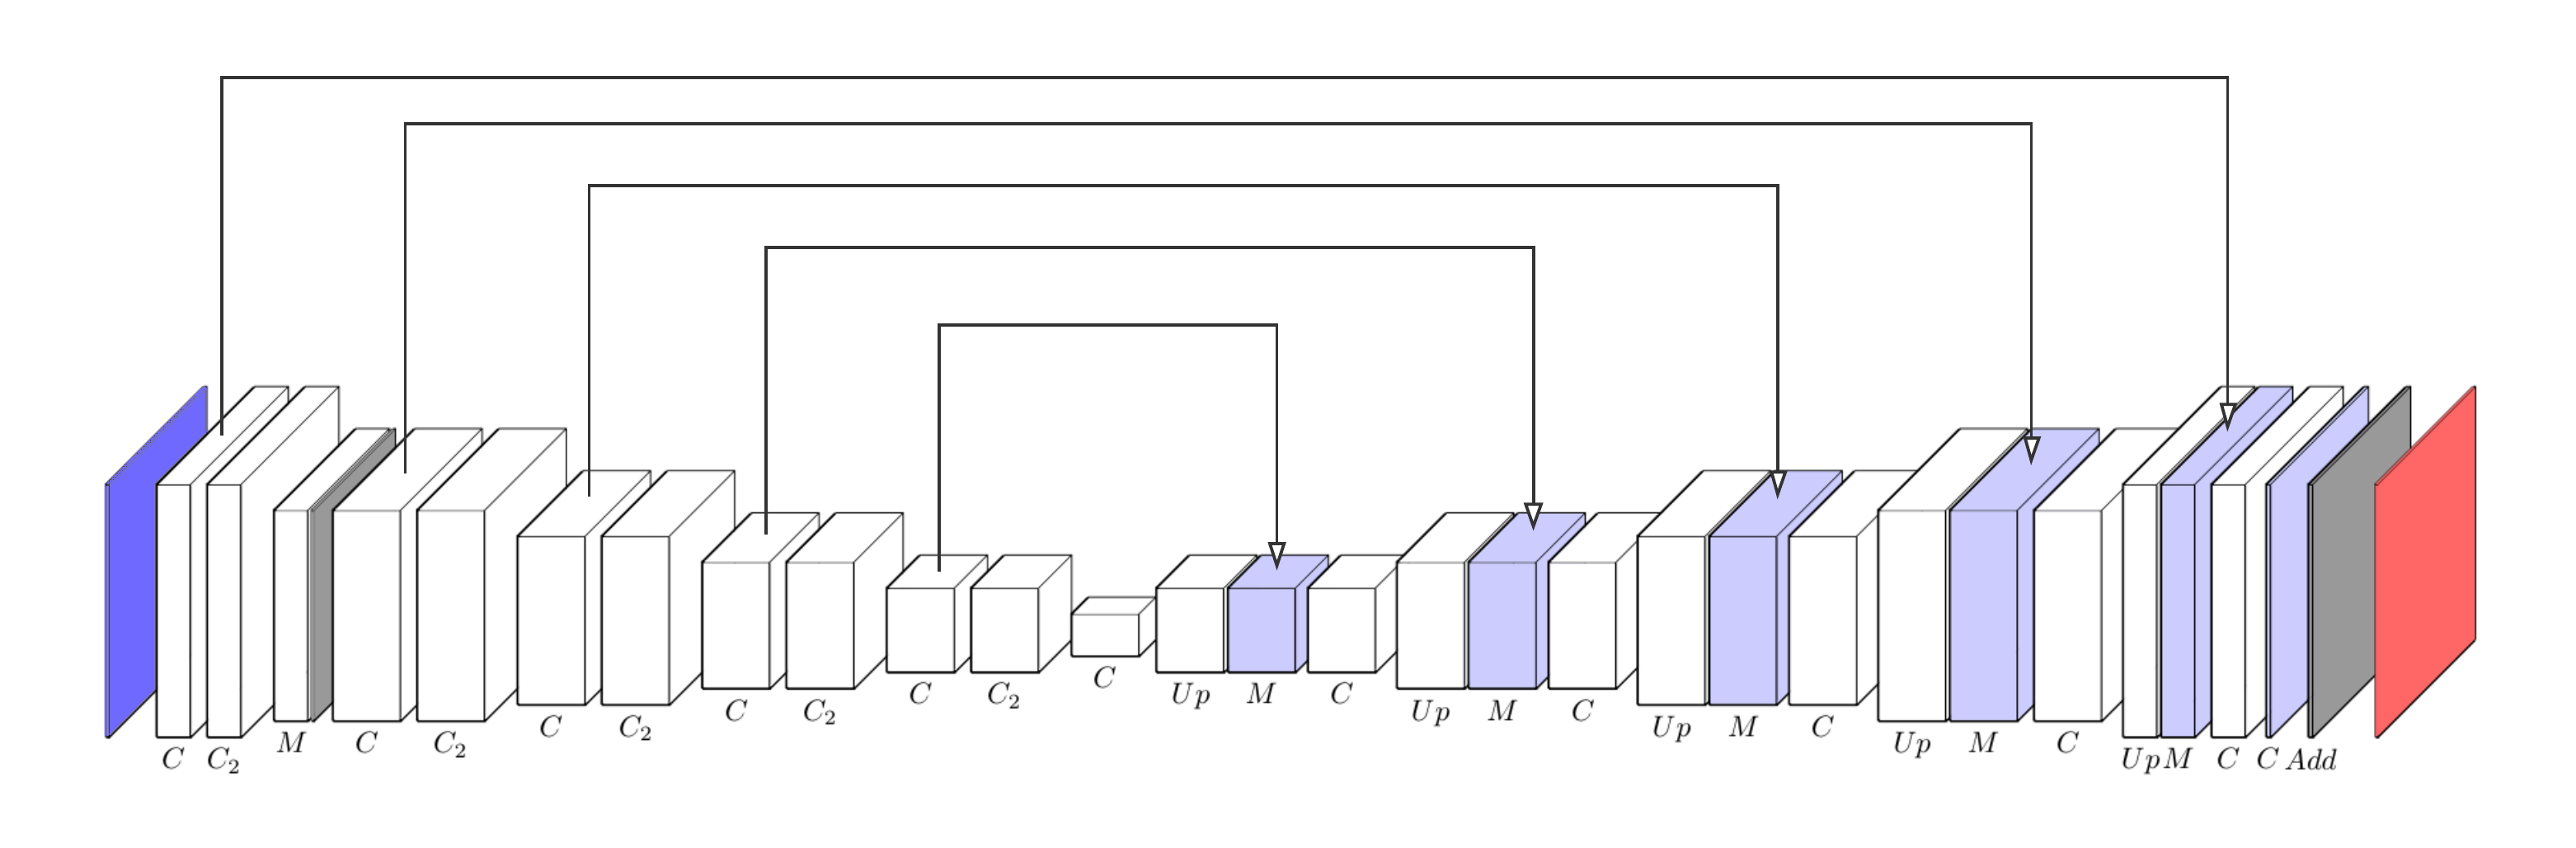
\includegraphics[width=\linewidth]{network}}
\caption{Network architecture for the human mask generation network. $C$ represents Convolutional layer and the subscript represents amount of stride. $M$ represents merge layer, $Up$ represents upsampling layer and $Add$ is the addition layer. }
\label{fig:net}
\end{figure*}
Our model is trained on (example, label) tuples of the form (($I_{s}$,$p_{s}$),$M_{t}$) where $I_{s}$, $p_{s}$ are the source image and its respective pose and $M_{t}$ is the target mask. The network architecture is demonstrated in ``Fig. \ref{fig:net}'' where the arrows denote the skip connections. The input to the model is the RGB image $I_{s} \in \mathbb{R}^{H\times W \times 3}$. The pose map $p_{s} \in \mathbb{R}^{H/2\times W/2\times 1}$ is concatenated in the second convolutional layer after downscaling it by 2. Contrary to \cite{pw} we do not represent each body part into as a separate layer for mask. Therefore, the output of the network is $\Delta M_{s} \in \mathbb{R}^{H\times W\times 1}$ is a single channel mask of the full human body. $\Delta M_{s}$ is added to an input prior mask (unlearned) $\hat M_{s}$ which specifies rough location of the person to be segmented. It is created in a similar manner the skeleton mask (see section \ref{gcm}) is created, but here the limbs are of gaussian distribution centered at the mid point of two joints. This helps in our model to converge to the segmentations we desire. Therefore, the final mask volume is \begin{equation} M_{s} = add (\Delta M_{s} + log(\hat M_{s})) \end{equation}. Kernel size $k$ is $3$ for all the convolutional layers except the first layer for which $k=7$. All the covolutional layers are followed by ``leaky Relu'' activation except the output layer which is followed by ``tanh'' activation.  

\subsubsection{Pre-processing}
The input to the network is centered, cropped and scaled in order to bring it to the desired size $(H_{d},W_{d})$ based on the bounding box of the person in focus. The same transformation is applied to the keypoints also and missing keypoints have coordinates $(0,0)$ and are ignored while creating the 2D gaussian posemap. After cropping and scaling source image ``$I_{s}$'' and ground truth mask ``$M_{t}$'' are normalized such that $I_{s}$, $M_{t} \in [-1,1]$. Data augmentation has not been done in the current experiments.

\subsubsection{Training}
The model has been trained on MS-COCO 2017 instance segmentation dataset with only person class. The model currently supports only single person in an image both for training and inference. In case of multiple person in one image, the same image can be supplied with different pose data consecutively. Therefore, for single person the model has been trained on about 60500 samples and validated on \ldots samples on 3 GB NVIDIA GTX-780 GPU, which has a compute capability of 3.5. Loss function was choosen to be MSE \textit{(Mean Squared Error)} with batch size fixed to 4 and ADAM Optimizer with learning rate $1e_{-4}$ for 30 epochs. The total training time on our machine with validation was about 90 hours. 

\section{Experiments and Results}
I evaluated the results on both MS-COCO 2017 validation set and about 100 single person images of the PASCAL VOC dataset. The dataset is quite diversified and thus has very less chance of overtraining. The input for the inference is only the RGB image and the 14 body keypoints. The input image dimension has been fixed to $256 \times 256 \times 3$. All the approaches have been evaluated on IOU \textit{(Intersection Over Union)} scores of the prediction and the ground truth mask. The problem with the ground truth of MS-COCO instance segmentation dataset is that the mask is not very pixel wise accurate and is a polygon mask instead. Therefore, the model is also not able to converge to a mask which is sharper at the boundary.

\subsection{Mask Refinement}
In order to produce a pixel-wise accurate mask, many techniques have been used in the past works like ``Atrous Convolutions'' (see section \ref{atr}), multiscale detection, Conditional Random Fields (see section \ref{CRF}) as post-processing in \cite{dpl1,dpl2}.
Details on how Atrous Convolution was experimented in our model is explained is Appendix \ref{atr-A}. Also, tuning the weights of the model with some samples of accurate ground truth is also a common approach in order to increase the accuracy score.

\subsubsection{Tuning using the VOC dataset}
PASCAL-VOC dataset has $20$ class instance segmentation dataset with $1753$ samples for person class in including train and validation set, out of which only about $500$ are single person images. From these $500$ images $435$ good quality images were selected for fine tuning the model and to also create an accurate validation set. Therefore, the selected samples are split with val/train ration of $0.25$. Keypoints are generated using \cite{poseAE} which gives 17 keypoints that do not include the head. Head is estimated and these keypoints are transformed into 14 keypoint array (see Appendix \ref{14_label}). The model is fine tuned on these images for $5$ epochs.Sample results have been shown in \ref{fig:re1}

\subsubsection{Fully Connected Conditional Random Fields}
There is always has been a trade-off between localization accuracy and classification performance in DCNNs. Its has been evident that very deep networks with multiple max-pooling layers improve the classification accuracy, but yields smooth responses. Many papers on semantic segmentation propose an approach based on coupling the recognition capacity of the DCNN and the fine-grained localization accuracy of fully connected CRFs to produce accurate segmentation results. 

Conditional Random Field is a specific type of graphical model. In our case it helps to estimate the posterior distribution given predictions from our network and raw RGB features that are represented by our image. It does that by minimizing the energy function which are defined by the user. In our case the effect is very similar to bilateral filter which takes into account the spatial closeness of pixels and their similarity in RGB feature space (intensity space). On a very simple level, it uses RGB features to make prediction more localized – for example the border is usually represented as a big intensity change – this acts as a strong factor that objects that lie on different side of this border belong to different classes. We implement CRF using a python package pydensecrf.
The scores obtained from the network are used as unary potentials for the CRF. The hyperparameters (refer Appendix ...) are optimized using a coarse-to-fine iterative grid search approach over some samples.

\begin{figure}[htbp]
\centering{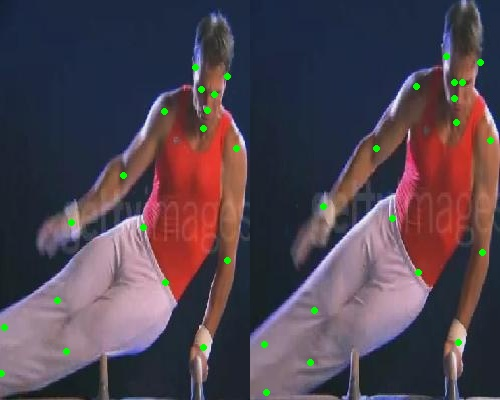
\includegraphics[width=0.9\linewidth]{dm1}}
\caption{ Keypoint Tracking in subsequent frames. \\ \textit{Left:} Reference frame, \textit{Right:} Query Frame.}
\label{fig:dm}
\end{figure}
\subsection{Results}
The output of the model without post processing using CRF is not binary as the last layer has ``tanh'' activation. Therefore, thresholding is done in order to binarize the output.
The IOU scores obtained on VOC and COCO test dataset of 100 images are mentioned in Table \ref{tab_final_results} for different experiments. The best score is obtained on the fine tuned model on VOC dataset with an IOU score of \ldots .

A comparison has also been done on other human parsing networks like JPP-Net and other state-of-the-art semantic segmentation networks. This is illustrated in Table \ref{tab_comp}. Our model clearly outperforms JPP-Net and gives comparable result against deeplab-v1. 
In terms of the number of parameters and inference time also our model outperforms deeplab-v1 with almost same accuracy score.

\begin{table}[htbp]
\caption{Table Type Styles}
\begin{center}
\begin{tabular}{|c|c|c|c|}
\hline
\textbf{Table}&\multicolumn{3}{|c|}{\textbf{Table Column Head}} \\
\cline{2-4} 
\textbf{Head} & \textbf{\textit{Table column subhead}}& \textbf{\textit{Subhead}}& \textbf{\textit{Subhead}} \\
\hline
copy& More table copy$^{\mathrm{a}}$& &  \\
\hline
\multicolumn{4}{l}{$^{\mathrm{a}}$Sample of a Table footnote.}
\end{tabular}
\label{tab1}
\end{center}
\end{table}


\begin{table}[htbp]
\caption{Table Type Styles}
\begin{center}
\begin{tabular}{|c|c|c|c|}
\hline
\textbf{Table}&\multicolumn{3}{|c|}{\textbf{Table Column Head}} \\
\cline{2-4} 
\textbf{Head} & \textbf{\textit{Table column subhead}}& \textbf{\textit{Subhead}}& \textbf{\textit{Subhead}} \\
\hline
copy& More table copy$^{\mathrm{a}}$& &  \\
\hline
\multicolumn{4}{l}{$^{\mathrm{a}}$Sample of a Table footnote.}
\end{tabular}
\label{tab1}
\end{center}
\end{table}

\section{Conclusion}

\section*{Acknowledgment}



\section*{References}

\begin{thebibliography}{00}
\bibitem{b1} G. Eason, B. Noble, and I. N. Sneddon, ``On certain integrals of Lipschitz-Hankel type involving products of Bessel functions,'' Phil. Trans. Roy. Soc. London, vol. A247, pp. 529--551, April 1955.
\bibitem{b2} J. Clerk Maxwell, A Treatise on Electricity and Magnetism, 3rd ed., vol. 2. Oxford: Clarendon, 1892, pp.68--73.
\bibitem{b3} I. S. Jacobs and C. P. Bean, ``Fine particles, thin films and exchange anisotropy,'' in Magnetism, vol. III, G. T. Rado and H. Suhl, Eds. New York: Academic, 1963, pp. 271--350.
\bibitem{b4} K. Elissa, ``Title of paper if known,'' unpublished.
\bibitem{b5} R. Nicole, ``Title of paper with only first word capitalized,'' J. Name Stand. Abbrev., in press.
\bibitem{b6} Y. Yorozu, M. Hirano, K. Oka, and Y. Tagawa, ``Electron spectroscopy studies on magneto-optical media and plastic substrate interface,'' IEEE Transl. J. Magn. Japan, vol. 2, pp. 740--741, August 1987 [Digests 9th Annual Conf. Magnetics Japan, p. 301, 1982].
\bibitem{b7} M. Young, The Technical Writer's Handbook. Mill Valley, CA: University Science, 1989.
\end{thebibliography}
\vspace{12pt}
IEEE conference templates contain guidance text for composing and formatting conference papers. Please ensure that all template text is removed from your conference paper prior to submission to the conference. Failure to remove the template text from your paper may result in your paper not being published.
IEEE conference templates contain guidance text for composing and formatting conference papers. Please ensure that all template text is removed from your conference paper prior to submission to the conference. Failure to remove the template text from your paper may result in your paper not being published.
IEEE conference templates contain guidance text for composing and formatting conference papers. Please ensure that all template text is removed from your conference paper prior to submission to the conference. Failure to remove the template text from your paper may result in your paper not being published.
IEEE conference templates contain guidance text for composing and formatting conference papers. Please ensure that all template text is removed from your conference paper prior to submission to the conference. Failure to remove the template text from your paper may result in your paper not being published.
\newpage
\onecolumn
\begin{appendices}
\section{}
lkasndkasndkl
\newpage
\section{}
\end{appendices}
\end{document}




